%
%
%

\section{Translational Parallel Handling Robots with Arbitrary Planar Rotation}
\label{sec:eval_handlingfreerotation}


%
%
%
%
%
%
%
%

A general handling task is taken as a second case study to investigate structures with 3T0R and 3T1R motion exemplarily.
Arbitrary planar rotation is allowed in the 3T0R task, which produces functional redundancy for 3T1R PRs.
The inverse-kinematics model for this case used in the dimensional synthesis is elaborated on in \cite{Schappler2022_ARK3T1R}.
The case study presents a simulative investigation without reference to an actual robot prototype, unlike in the previous section.
A similar evaluation has been published in \cite{Schappler2022_ARK3T1R} in preliminary form.
In Section~\ref{sec:eval_handling_task}, the requirements, based on the paper \cite{PrauseChaCor2015}, are summarized and formalized within the synthesis framework.
The results are introduced in Section~\ref{sec:eval_handling_results}, followed by the evaluation of functional redundancy in Sections~\ref{sec:eval_handling_results_taskred}--\ref{sec:eval_handling_results_taskred_general}, a comparison to the reference work~\cite{PrauseChaCor2015} in Section~\ref{sec:eval_handling_results_reference_comparison} and the summary in Section~\ref{sec:eval_handling_summary}. %
%


%
%
%
%
%
%
%
%
%


\subsection{Task Requirements}
\label{sec:eval_handling_task}


%
%
%
%
%
%
%
%
%

By reproducing the requirements of the case study from \cite{PrauseChaCor2015}, a validation of this thesis' synthesis framework against the one from \cite{Prause2016} is performed (cf. Section~\ref{sec:ds_combstructgeomsynth}).
The requirements are summarized in Table~\ref{tab:handling_constraints}.
\emph{The task} is specified as a \emph{reachable cuboid workspace} of \SI{200}{\milli\metre} $\times$ \SI{200}{\milli\metre} $\times$ \SI{100}{\milli\metre}.
A visualization is given in Figure~\ref{fig:handlingpkm_robots_selection} with some of the robot structures.
By sampling each dimension with three values, 27 \emph{reference points} are defined. 
The orientation is not specified for 3T1R robots, which permits choosing it by~optimization.

\begin{figure}[H]
  \begin{adjustwidth}{-\extralength}{0cm}
    \centering
    \graphicspath{{Figures}}
    \input{./Figures/handlingpkm_robots_selection.pdf_tex}
  \end{adjustwidth}
  \caption{Visualization %
  %
    of selected results for the handling task from the \propername{Pareto} diagrams in Figure~\ref{fig:handlingpkm_pareto}.}
  \label{fig:handlingpkm_robots_selection}
\end{figure}



\newcounter{handlingconstraints}
\begin{table}[H]
  \caption[Constraints and parameter limits for the handling task]{Constraints and parameter limits for the handling task with reference to numbers in Section~\ref{sec:materials}}
  \begin{adjustwidth}{-\extralength}{0cm}
    \centering
    \label{tab:handling_constraints}	
    \begin{tabularx}{\fulllength}{CcCc}
      \toprule
      \textbf{\#} & \textbf{Constraint} & \textbf{Section~\ref{sec:ds_constraints}} &  \textbf{Value} \\
      \midrule
      \refstepcounter{handlingconstraints}\thehandlingconstraints\label{handlingconstr:installspace} & \makecell{installation space (depending\\ on joint index in the chain)} & no.~\ref{itm:constr_installspace} & \makecell{joints 1--3 not above lower workspace limit,\\ joints 4--5 not above upper workspace limit} \\		
      \midrule
      \refstepcounter{handlingconstraints}\thehandlingconstraints\label{handlingconstr:prismaticrange} & prismatic joint stroke length & no.~\ref{itm:constr_jointrange}  & max. \SI{400}{\milli\metre} \\
      \midrule
      \refstepcounter{handlingconstraints}\thehandlingconstraints\label{handlingconstr:legchainlength} & length of a leg chain & no.~\ref{itm:constr_jointrange} & max. \SI{1000}{\milli\metre} \\
      \midrule
      \refstepcounter{handlingconstraints}\thehandlingconstraints\label{handlingconstr:baselim} & base diameter & no.~\ref{itm:constr_param_radius}  &  200--1000 mm \\
      \midrule
      \refstepcounter{handlingconstraints}\thehandlingconstraints\label{handlingconstr:plflim} & platform diameter & no.~\ref{itm:constr_param_radius} &  200--1000 mm, smaller than base \\	
      \midrule
      \refstepcounter{handlingconstraints}\thehandlingconstraints\label{handlingconstr:poserr} & precision (position error) & no.~\ref{itm:constr_obj} &  max. \SI{0.5}{\milli\metre} (for objective~\ref{itm:obj_poserr} in Section~\ref{sec:ds_objective})\\
      \midrule
      \refstepcounter{handlingconstraints}\thehandlingconstraints\label{handlingconstr:condition} & \propername{Jacobian} condition number  & no.~\ref{itm:constr_ik_sing} &  \gape{max. $10^4$ (IK and manipulator \propername{Jacobian})}\\
      \midrule
      & \textbf{Parameter} & \textbf{Section~\ref{sec:dimsynth_optvars}} &  \textbf{Value} \\
      \midrule
      \refstepcounter{handlingconstraints}\thehandlingconstraints\label{handlingconstr:baseposition_z} & vertical base position in $\rovec{\indks{W}}{0}$ & no.~\ref{itm:param_basepos} & 1--0.1 m below the task \\
      \midrule
      \refstepcounter{handlingconstraints}\thehandlingconstraints\label{handlingconstr:baseposition_xy} & base position in $x$-$y$-plane & no.~\ref{itm:param_basepos} & 0 (no optimization) \\
      \midrule
      \refstepcounter{handlingconstraints}\thehandlingconstraints\label{handlingconstr:param_baseori} & \gape{base rotation $\rotmat{\indks{W}}{0}$} & no.~\ref{itm:param_baseori} & $\varphi_{\mathrm{b},x}~{=}~\varphi_{\mathrm{b},y}~{=}~0$ and $\varphi_{\mathrm{b},z}{\in}[-\SI{180}{\degree},\SI{180}{\degree}]$\\
      \midrule
      \refstepcounter{handlingconstraints}\thehandlingconstraints\label{handlingconstr:param_basejointincl} & base-joint inclination $\gamma_{\mathrm{b}}$ & no.~\ref{itm:constr_param_inclination} & $\SI{5}{\degree} < \gamma_{\mathrm{b}} < \SI{30}{\degree}$ (for conic alignment)\\
      \midrule
      \refstepcounter{handlingconstraints}\thehandlingconstraints\label{handlingconstr:ee_translation} & end-effector translation $\rovec{\indks{P}}{\indks{E}}$ & no.~\ref{itm:param_eepos} & [0,\,0,\,0] (no optimization) \\	
      \midrule
      \refstepcounter{handlingconstraints}\thehandlingconstraints\label{handlingconstr:param_eeori} & \gape{end-effector orientation $\rotmat{\indks{P}}{\indks{{E}}}$} & no.~\ref{itm:param_eeori} & $\varphi_{\mathrm{p},x}=\varphi_{\mathrm{p},y}=\varphi_{\mathrm{p},z}=0$ (no opt.)\\
      \midrule
      & \textbf{Load} &  &  \textbf{Value} \\
      \midrule
      \refstepcounter{handlingconstraints}\thehandlingconstraints\label{handlingconstr:forces} & maximal external forces &  &  \gape{$\ortvek{W}{f}{\transp}{\mathrm{ext}}=$ [2,\,2,\,$-$10] \SI{}{\newton}}  \\
      \bottomrule
    \end{tabularx}
  \end{adjustwidth}
\end{table}

The combined structural and dimensional synthesis in \cite{PrauseChaCor2015} is based on the 27 reference points, and results for 3T0R PRs with prismatic actuation are obtained using a single-objective optimization. %
There, a detailed investigation of the best parameterization for all structures is performed with a finer discretization of \SI{10}{\milli\metre} in each dimension and, thereby, 4851 points.
Since the proposed framework can handle this complexity, a \emph{reference path} connecting the 4851 points in a zigzag motion (by the same number of samples) is used directly within the synthesis of this study after the check of the 27 reference points.
Thereby, the risk of unreachable parts within the workspace decreases.
For 3T1R robots, dynamic programming (cf. \cite{Schappler2023_ICINCOLNEE}) is used for optimizing the redundant rotational \hl{DoF} with twelve stages and five states %
and a limitation of $\pm$\SI{60}{\degree} around the initial value, resulting from the IK optimization.

Only the force transmission, without statics or dynamics, is considered, as in \cite{PrauseChaCor2015}.
The \emph{robot and payload mass are neglected}, which allows the use of the simplified \emph{trajectory} with discontinuous velocity and acceleration profiles by numeric differentiation.
The actuator force is computed based on a given external force (corresponding to a payload of \SI{1} kg, cf. row~\ref{handlingconstr:forces} in Table~\ref{tab:handling_constraints}) and used as an objective (number~\ref{itm:obj_maxactforce} in Section~\ref{sec:ds_objective}), as in \cite{PrauseChaCor2015}.
As a second additional objective (number~\ref{itm:obj_installspace} in Section~\ref{sec:ds_objective}), the installation space is used to be able to select robots with a good ratio of (fixed) workspace to (optimized) installation space.
The precision (number~\ref{itm:obj_poserr} in Section~\ref{sec:ds_objective}) was selected as a third criterion for further exploration of the solution space as it conflicts with the actuator force by lever effects.


\begin{figure}[H]
  \begin{adjustwidth}{-\extralength}{0cm}
    \centering
    \begin{overpic}
      {Figures/handlingpkm_pareto_actforce_installspace_groups_default_prismatic.pdf}
      \put(0,0){(\textbf{a})}
    \end{overpic}\\[5mm]
    \begin{overpic}
      {Figures/handlingpkm_pareto_actforce_installspace_groups_default_revolute.pdf}
      \put(0,0){(\textbf{b})}
    \end{overpic}
  \end{adjustwidth}
  \caption{\propername{Pareto} fronts for robots with (\textbf{a}) prismatic and (\textbf{b}) revolute actuation. The notation of \cite{KongGos2007} is used for distinguishing kinematic structures, where {two} \`R denote two parallel revolute joints and \'R denotes {a} joint with a different axis.
    {In addition to \cite{KongGos2007}, prismatic joints with an axis parallel to a revolute \`R joint are denoted by \`P.}}
  \label{fig:handlingpkm_pareto}
\end{figure}
Several geometric \emph{constraints} are set to increase the practicability of the solutions. 
A floor-mounted PR is assumed to simplify the visualizations contrary to the more practical existing ceiling-mounted robots.
The robot structure should be below the workspace (row~\ref{handlingconstr:installspace}) to avoid impractical crane-like designs.
Further constraints are taken from \cite{PrauseChaCor2015}, such as a limited prismatic joint stroke (row~\ref{handlingconstr:prismaticrange}), chain length (row~\ref{handlingconstr:legchainlength}), and base and platform diameters (rows~\ref{handlingconstr:baselim} and~\ref{handlingconstr:plflim}).
The required joint-coordinate range of prismatic joints in the chain (realized by lifting cylinders) results in 400--800 mm by constraint no.~\ref{itm:constr_prismaticcylinder} from Section~\ref{sec:ds_constraints}.
To avoid singularities and to obtain feasible handling performance, e.g., in industrial pick-and-place tasks, the end-effector precision (row~\ref{handlingconstr:poserr}) was additionally limited to \SI{500}{\micro\metre}, which is {achieved by} all results from \cite{PrauseChaCor2015} {(Figure~\ref{fig:handlingpkm_boxplot_PrauseChaCor2015}d in Appendix~\ref{sec:app_handlingpkm})} and %
%
does not deteriorate the comparability.
The encoder error of \SI{52}{\micro\metre} from \cite{PrauseChaCor2015} was used for prismatic actuation and \SI{7}{\arcsecond} from \cite{HeidenheinEncoder} for revolute actuation.
For further exclusion of near-singular PRs (\mbox{types~I and~II}), \propername{Jacobian} condition-number limits are set (row~\ref{handlingconstr:condition}).
The robot base is assumed below the center of the workspace (rows~\ref{handlingconstr:baseposition_z} and~\ref{handlingconstr:baseposition_xy}) with further optimization of the base rotation (row~\ref{handlingconstr:param_baseori}).
No end-effector transformation is assumed (rows~\ref{handlingconstr:ee_translation} and~\ref{handlingconstr:param_eeori}), and only an offset distance is used for visualization, e.g., in Figure~\ref{fig:handlingpkm_robots_selection}.

In \cite{PrauseChaCor2015}, only robots with tangential (``triangular'') and conical (``star-shaped'') \emph{base-joint alignment} are considered as showcases.
This restriction is lifted in the following, and all other structures (radial and vertical base joints) are allowed to increase the number of results and show the variety of produced solutions by the proposed framework.
Only the restriction on the conical base joints' elevation of \cite{PrauseChaCor2015} is maintained (row~\ref{handlingconstr:param_basejointincl}) for~compatibility.


The synthesis is performed for all 3T0R and 3T1R PRs from a previous structural synthesis {with actuation} of the first revolute or single prismatic joint.
In total, 329 variants (combinations of leg chains and base- and platform-coupling\hl{-}joint alignments) are investigated, 239 for 3T0R and 90 for 3T1R.
Of these, 226 match the requirements (200 for 3T0R and 26 for 3T1R).
The results are summarized into 36 groups of 3T0R (25 prismatic and 11 revolute actuation) and 12 groups of 3T1R (5 prismatic, 7 revolute actuation) by their respective leg chain.
The results for all coupling-joint alignments for one leg chain are summarized into one \propername{Pareto} front, similar to the case study in Section~\ref{sec:eval_water}.

The particle swarm optimization for 7 to 13 parameters (depending on the structure) is configured similarly as before, with 400 individuals and a time limit of \SI{10}{\hour} with a computation time of up to 20--40 s for 3T0R and \SI{2}{\minute} for 3T1R robots, depending on the abortion due to constraint violation.
The longer computation time for 3T1R robots results from the more complex model (one additional chain), more possibility for assembly modes, and especially, the redundancy resolution.
Several optimization iterations are performed in which constraints are added and refined, and intermediate results are taken as initial values for the successive iterations.

\subsection{Overview of the Synthesis Results}
\label{sec:eval_handling_results}

%
%
%
%
%
%


The optimization results are depicted in Figure~\ref{fig:handlingpkm_pareto} in \propername{Pareto} fronts separately for prismatic and revolute actuation due to the different units and clarity.
Four exemplary robot structures are shown in Figure~\ref{fig:handlingpkm_robots_selection}.
The remainder of the structures are visualized in Appendix~\ref{sec:app_handlingpkm} in Figures~\ref{fig:handlingpkm_robots_3T0R_rev1}--\ref{fig:handlingpkm_robots_reference} with parameters in Tables~\ref{tab:handlingpkm_results_pris}--\ref{tab:handlingpkm_results_rev_dh}.

For \emph{prismatic actuation} in Figure~\ref{fig:handlingpkm_pareto}a, many different structures show a comparably good performance; however, the
\hyperrefl{restabrow:P3PRRRR7V1GxPxA1}{3-\underline{P}{U}{R}{R}} (Figure~\ref{fig:handlingpkm_robots_3T0R_pris1}h),  \hyperrefl{restabrow:P3PRRRR8V1GxPxA1}{3-\underline{P}{U}{U}} (linear Delta, Figure~\ref{fig:handlingpkm_robots_selection}c), and \hyperrefl{restabrow:P3PRRRR8V2GxPxA1}{3-\underline{P}RRU} (variant 2, Figure~\ref{fig:handlingpkm_robots_3T0R_pris1}k) clearly outperform the other solutions regarding the selected criteria.
The \hyperrefl{restabrow:P3PRRRR7GxPxA1}{3-\underline{P}{R}{\`R}{\`R}{\`R}} (Figure~\ref{fig:handlingpkm_robots_3T0R_pris1}g) and \hyperrefl{restabrow:P3PRRRR8GxPxA1}{3-\underline{\`P}{\`R}{\'R}{\'R}{\`R}} (Figure~\ref{fig:handlingpkm_robots_3T0R_pris1}i) show similar performance, as they correspond to the same robots but with universal joints expanded to single revolute joints.
The 3T1R structures require a significantly higher actuator force of about \SI{10}{\newton} (e.g.,~\hyperrefl{restabrow:P3RPRRR8V3GxPxA2}{4-{\`R}\underline{P}{\`R}{\'R}{\'R}}, Figure~\ref{fig:handlingpkm_robots_selection}d) compared to \SI{4}{\newton} (Figure~\ref{fig:handlingpkm_pareto}a) for a similar installation space.


For the \emph{revolute actuation} in Figure~\ref{fig:handlingpkm_pareto}b, the \hyperrefl{restabrow:P3RRRRR6V1GxPxA1}{3-\underline{R}{U}{R}{R}} (Figure~\ref{fig:handlingpkm_robots_3T0R_rev1}g) performs best, followed by the Delta robot structure (\hyperrefl{restabrow:P3RRRRR10V1GxPxA1}{3-\underline{R}{U}{U}}, Figure~\ref{fig:handlingpkm_robots_selection}a) and variants thereof.
The Delta's base-joint alignment is chosen unconventionally by a radial drive axis.
The ability of this alignment to support the established Delta robot construction using a spatial parallelogram needs further investigation before eventual realization.
The relative disadvantage of 3T1R structures is similar to prismatic actuation of about 100\% regarding the actuator force/torque of the best 3T0R structure.
The 3T1R \hyperrefl{restabrow:P4RRRRR10V1GxPxA1}{4-\underline{R}{U}{U}} (Figure~\ref{fig:handlingpkm_robots_selection}b), for instance, and the \hyperrefl{restabrow:P4RRRRR5V1GxPxA1}{4-\underline{R}{R}{U}{R}} (Figure~\ref{fig:handlingpkm_robots_3T1R_rev}e), e.g., require \SI{3}{\newton\metre} and \SI{2}{\newton\metre} actuator torque compared to \SI{1}{\newton\metre} for the 3T0R \hyperrefl{restabrow:P3RRRRR6V1GxPxA1}{3-\underline{R}{U}{R}{R}}.


\subsection{Comparison to Results from the Literature and Evaluation of the Framework}
\label{sec:eval_handling_results_reference_comparison}

The structures from \cite{PrauseChaCor2015} are evaluated in Figure~\ref{fig:handlingpkm_pareto}a as an additional benchmark if they exist in the database.
Structures with both prismatic (P) and cylindrical (C) joints are omitted since this corresponds to two prismatic DoFs (one passive) within one leg chain.
%
A rather exact reproduction of the actuator forces from \cite{PrauseChaCor2015} was possible for the 3-\underline{C}RR, 3-\underline{P}UU, and 3-U\underline{P}U using the parameters from the paper, as is visible in a comparison of the box plots from \cite{PrauseChaCor2015}, cf. Figure~\ref{fig:handlingpkm_boxplot_PrauseChaCor2015}.
For the 3-\underline{C}UR and 3-\underline{C}RU, the values were in the same range but with a different distribution over the 4851 trajectory samples.
The difference is already contained within the \propername{Jacobian}, which differs between the robot assembly modes, visible in Figure~\ref{fig:handlingpkm_boxplot_PrauseChaCor2015}e--f.
In conclusion, the \emph{kinetostatic model} is likely consistent.
Still, the reference's collision model (if any) and the selection strategy of the assembly mode may explain the deviation using the same kinematic parameters.
%
%

The markers from \cite{PrauseChaCor2015} are dominated by the corresponding \propername{Pareto} fronts (using the same marker symbol but a different color).
Due to the complexity of the \emph{optimization problem}, a possible reason is hard to determine.
The additional use of the reference trajectory does not explain the difference  from \cite{PrauseChaCor2015}, where results are only based on the 27 reference points, as the optimization only based on these 27 reference points leads to qualitatively similar results as Figure~\ref{fig:handlingpkm_pareto}a, shown in appendix Figure~\ref{fig:handlingpkm_pareto_prismatic_onlypoints}.
Next to the differences mentioned above, one other reason could be an undocumented further constraint in the paper or the underlying framework of the PhD thesis \cite{Prause2016}.
An influence that is not less likely is the insufficient exploration ability of the employed single-objective genetic algorithm from \cite{MatlabGOT} instead of the PSO, which was also observed (for the multi-objective variant) in the case study~\cite{SchapplerJahRaaOrt2022}.


\subsection{Evaluation of Functional Redundancy of 3T1R Parallel Robots}
\label{sec:eval_handling_results_taskred}

Although symmetric 3T1R PRs do not reach as low actuator forces as their 3T0R counterparts, their principal operational capability presents an interesting result compared to the state of the art, where mostly theoretical structures are shown.
They benefit from the redundancy resolution using dynamic programming (see \cite{Schappler2023_ICINCOLNEE}). %

In Figure~\ref{fig:handlingpkm_perfmap_traj}b, an illustrative performance map is given for the \hyperrefl{restabrow:P4RPRRR8V2GxPxA2}{4-{R}\underline{P}{U}{R}} (Figure~\ref{fig:handlingpkm_robots_3T1R_pris}\,b).
This heat-map representation of the redundant degree of freedom over the trajectory was introduced by Wenger (see \cite{RevelesWenoth2016}) and is discussed in \cite{Schappler2023_ICINCOLNEE} in more detail.
The actuator-force representation in the map color corresponds to the objective of the IK optimization. 
It provides a direct interpretation in this case study since only the transmission of the given external force is considered, and rigid-body dynamics are neglected.
Within the optimization of the planar rotation coordinate, the maximal force of any of the actuators is minimized to 
5.3--12.2 N by avoiding orientations with higher forces. %
The upper bound is taken as objective (number~\ref{itm:obj_maxactforce} in Section~\ref{sec:ds_objective}) in Figure~\ref{fig:handlingpkm_pareto}.
For reference, the position trajectory is given in Figure~\ref{fig:handlingpkm_perfmap_traj}a, showing the zigzag motion of the $x$ and $y$ coordinates while ascending in the $z$ coordinate and, thereby, sampling the cuboid workspace.
The actuator-force/-torque performance maps of the other 3T1R PRs are given in appendix Figure~\ref{fig:handlingpkm_perfmaps_multi_actforce_pris} and~\ref{fig:handlingpkm_perfmaps_multi_actforce_rev}.
There, avoiding constraint violations (singularities, collisions, accuracy) dominates the force objective within the motion due to the relatively homogeneous pose-independent transmission ratio of the given external force (regarding the most-stressed actuator).
The evaluation already shows that the redundancy-resolution scheme from \cite{Schappler2023_ICINCOLNEE} also provides plausible results for 3T1R PRs regarding the optimality of the trajectory of the redundant~coordinate. 

\vspace{3pt}
\begin{figure}[H]
  \centering %
  \begin{adjustwidth}{-\extralength}{0cm}
    \begin{overpic}%
      {Figures/handlingpkm_trajectory.pdf} %
      \put(107,0){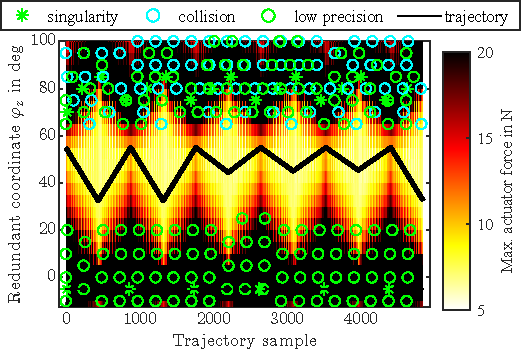
\includegraphics{Figures/handlingpkm_perfmaps_detail_P4RPRRR8V2G_actforce_maxactforce.pdf}} %
      \put(0,0){(\textbf{a})}
      \put(107,0){(\textbf{b})}
    \end{overpic}
  \end{adjustwidth}
  \caption{Trajectory
    of end-effector position (\textbf{a}) and of the planar rotation (redundant coordinate) within the force performance map with markers for constraint violation (\textbf{b}) for the 4-{R}\underline{P}{U}{R}.} %
  \label{fig:handlingpkm_perfmap_traj}
\end{figure} 

\textls[15]{The inspection of performance maps for other criteria in Figures~\ref{fig:handlingpkm_perfmaps_multi_poserr_pris}--\ref{fig:handlingpkm_perfmaps_multi_condikjac_rev} shows possible disadvantages of the symmetric 3T1R PRs compared to 3T0R PRs, even though all constraints are met within the results of the \propername{Pareto} front.
  The position error is much higher for prismatic actuation, except for the  \hyperrefl{restabrow:P4PRRRR6V1GxPxA1}{4-\underline{P}{R}{U}{R}} (Figure~\ref{fig:handlingpkm_robots_3T1R_pris}a), cf.~Figure~\ref{fig:handlingpkm_perfmaps_multi_poserr_pris}a.
  Many 3T1R PRs with revolute actuation exhibit IK singularities within the workspace, which is not possible to detect or avoid numerically with the \SI{10}{\milli\metre} trajectory sampling and the chosen approach of discretely evaluating the condition number, as, e.g., visible in Figure \ref{fig:handlingpkm_perfmaps_multi_condikjac_rev}b,f,g).
  Therefore, special attention must be paid to this aspect to investigate the structures further.}


The objective of the inverse kinematics influences the motion of the platform rotation, provided that the constraints leave sufficient space for optimization.
An example of the trajectories resulting from different IK objectives is given in Figure~\ref{fig:handlingpkm_pareto_compare_ik_obj}a for a parameterization of the \hyperrefl{restabrow:P4RPRRR8V2GxPxA2}{4-{R}\underline{P}{U}{R}} with radially aligned base-coupling joints (unlike in Figure~\ref{fig:handlingpkm_robots_3T1R_pris}b).
The precision is chosen as map color as it also highlights singularities.
Repeating the variation of the IK objective for each point of the robot's \propername{Pareto} front from the optimization (termed ``heuristic'') and evaluating the objective functions leads to a new \propername{Pareto} front for each of the IK objectives, shown in Figure~\ref{fig:handlingpkm_pareto_compare_ik_obj}b--c.
Therefore, the selection of the IK objective indirectly influences the performance of the dimensional synthesis.
Using the same objectives for the IK redundancy resolution and the dimensional synthesis provides the most promising results and corresponds best to the principle of bilevel optimization.
In the specific example of Figure~\ref{fig:handlingpkm_pareto_compare_ik_obj}b, the precision can be reduced by approximately 5\% against the constant-orientation case and 10\% against the heuristic approach of a weighted sum of several objectives, depending on the objectives and constraints of the dimensional synthesis.
The approach does not provide significant improvement for the installation-space objective, as visible in Figure~\ref{fig:handlingpkm_pareto_compare_ik_obj}c.
Other examples (case studies or robots) show qualitatively similar results.
The extent of possible improvement depends on the objectives of the dimensional synthesis and the IK settings that were used to obtain the results, as well as on the robot and task~requirements.

\begin{figure}[H]
  \begin{adjustwidth}{-\extralength}{0cm}
    \begin{overpic}%
      {Figures/handlingpkm_perfmap_compare_ik_obj_P4RPRRR8V2G3P1A1_p1.pdf} %
      \put(101,0){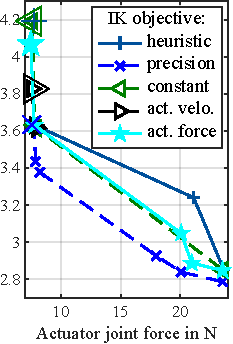
\includegraphics{Figures/handlingpkm_pareto_actforce_positionerror_compare_P4RPRRR8V2G3P1A1_p1.pdf}} %
      \put(142,0){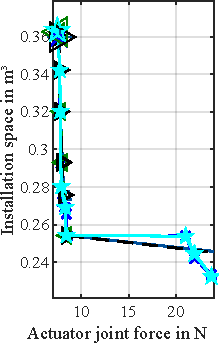
\includegraphics{Figures/handlingpkm_pareto_actforce_installspace_compare_P4RPRRR8V2G3P1A1_p1.pdf}}
      \put(0,2){(\textbf{a})}
      \put(98,2){(\textbf{b})}
      \put(140,2){(\textbf{c})}
    \end{overpic}
  \end{adjustwidth}
  \caption{Redundant-coordinate trajectory (\textbf{a}) and \propername{Pareto} fronts (\textbf{b},\textbf{c}) for another 4-{R}\underline{P}{U}{R} structure based on the same parameters with different inverse-kinematics optimization objectives. The method legend in (\textbf{b}) holds for all (\textbf{a}--\textbf{c}). Large markers in~(\textbf{b},\textbf{c}) represent parameters for the performance map in~(\textbf{a}).} %
  \label{fig:handlingpkm_pareto_compare_ik_obj}
\end{figure} 


%
%
%

%
%


\subsection{Discussion of Redundancy Resolution Within the Dimensional Synthesis}
\label{sec:eval_handling_results_taskred_general}

The downside of possible improvements by redundancy resolution is that the (multi-objective) dimensional synthesis optimization results are based on the (single-objective) redundancy-resolution method.
The performance of the synthesis {with one setting} can then not be obtained by other IK settings.
This overfitting can be avoided by using generic or no IK objectives (e.g., constant orientation or minimal platform motion) with little degree of freedom (e.g., few states in the dynamic programming) at the cost of lower performance in the synthesis objectives.
%
%
%
%
By these results and considerations, the two underlying assumptions of the paper regarding dimensional synthesis and functional redundancy can be addressed: %

%
%
%
%
%
%
\begin{Assumption}
  Optimizing the objective of the dimensional synthesis in an inner-loop redundancy resolution improves the synthesis results in the case of functional redundancy.
\end{Assumption}

%
%
An improvement of the synthesis objective by up to 10\% was shown for some examples.
Therefore, the proposed inner loop  ``\emph{is likely to improve the synthesis results}''. 
As the effect varies, the assumption may not hold in all cases or can not be tested generally (for the complete \propername{Pareto} front, all tasks, and all robot structures).

A thorough statistical evaluation for greater generality would require a metric for comparison of \propername{Pareto} fronts.
This is aggravated by the fact that the density of particles on the front is imbalanced, and gaps in the front are sometimes due to impossibility by constraint violations, sometimes by insufficient exploration.
The true form of the front is thereby unknown and only sampled incompletely by the heuristic optimization algorithm.
%
Quantifying the effect in a single-objective optimization would be easier from a methodological point of view.
However, it would also be less valuable, as a trade-off between multiple objectives has to be found for an actual robot design.
%
This leads to

\begin{Assumption} For a meaningful comparison including functionally redundant robots, the redundancy resolution has to be performed within the dimensional synthesis. Only then can the dominance (outperformance) of one structure compared to another be determined.
\end{Assumption}
%
%
%

\newpage
The redundancy resolution should be used to avoid constraint violations and receive feasible results in the first place.
Without using the redundancy at all, too many particles (i.e., sets of kinematic parameters) would be unnecessarily discarded for constraint violation, which would deteriorate the results.
The assumption can be \emph{argued to be true if redundancy resolution is only defined as avoiding constraint violation} and having no influence otherwise (i.e., leaving the redundant coordinate constant or using some shortest-distance metric for optimization beyond the constraints).

Furthermore, optimizing for a general objective for \emph{the initial poses of the reference trajectory} proved to be a promising approach. %
This may be influenced by the fact that most of the \propername{Pareto}-optimal performance maps could be traversed well with constant orientation, and the performance distribution over the redundant coordinate did not change much.
It can be assumed that this was not induced by the synthesis (i.e., self-fulfilling by overfitting) since the redundancy resolution was also proven to cope with other, more complicated cases.
For the synthesis of other trajectories, %
this could already be different, and the initial pose may have less influence as extensive nullspace motion would be necessary regardless.
%
Thereby, from the results obtained so far, the assumption \emph{is not likely valid for understanding redundancy resolution as initial-pose optimization}.

The assumption also does \emph{not hold when understanding redundancy resolution as optimization within the reference trajectory} since several further assumptions have to hold, depending on the use case.
In multi-objective optimization, the non-redundancy-optimized solution may present a compromise solution, and the optimized solution may be better in one objective but worse in the other objectives and, therefore, not \propername{Pareto}-dominant.
The extent of this effect depends on the selection of objectives and their respective opposition.
Optimizing the inverse kinematics for one objective in the design phase may lead to overfitting, and using the structure later with a different IK objective may present worse results.
Therefore, the priority of the objectives and the aversion to this overfitting would have to be defined beforehand for the assumption to be true without restrictions. %


\subsection{Summary of the Case Study}
\label{sec:eval_handling_summary}

The numerous theoretical results show the efficiency of the synthesis approach for this general 3T0R task. %
The results for functional redundancy show, in principle, that reasonable solutions exist and a comparison is feasible. %
However, the performance of redundant structures is weaker than that of non-redundant. %
The 3T1R structures may still perform better for other objectives, which should be evaluated if a task-specific synthesis is performed.
However, due to the simplicity of the 3T0R structures, the advantage of the 3T1R structures to avoid collisions and singularities may not be relevant since 3T0R robots, such as the Delta robot, do not suffer widely from singularities or self-collisions within the workspace.
%
By direct comparison to the results of \cite{PrauseChaCor2015}, parts of the methodology could be validated for the 3T0R case.

